\chapter{Espectroscopia rotacional e vibracional}\label{ch:b3:rovibrational-spectroscopy}

Em um planalto alto e seco, dezenas de antenas de rádio apontam para uma nuvem
escura entre as estrelas. Entre as frequências que elas captam está uma em
\qty{115.271}{GHz}: moléculas de monóxido de carbono, a alguns kelvins,
passando de seu primeiro nível rotacional para o mais baixo. Desse único
número um químico obtém o comprimento da ligação C--O a uma fração de
picômetro; das intensidades das raias seguintes, a temperatura da nuvem. As
rotações e vibrações das moléculas são o tema deste capítulo: seus níveis,
a partir do rotor e do oscilador do \cref{ch:b3:quantum-model-systems}; as
regras de seleção, a partir do \cref{ch:b3:group-theory-applied}; e o que os
espectros medem --- comprimentos de ligação, \omterm{def:b3:quantum-model-systems:oscillator}{constantes de força}, energias
de dissociação.

\begin{recall}
O \cref{ch:b3:quantum-model-systems} deu o \omterm{def:b3:quantum-model-systems:rotor}{rotor rígido}, $E_J = J(J+1)\hbar^2/2I$
com \omterm{def:b3:quantum-model-systems:degenerate}{degenerescência} $2J + 1$, e o \omterm{def:b3:quantum-model-systems:oscillator}{oscilador harmônico}, $E_v = (v + \frac12)h\nu$,
para uma diatômica de \omterm{def:b3:quantum-model-systems:oscillator}{massa reduzida} $\mu$. O \cref{ch:b3:group-theory-applied}
enunciou as regras de seleção no infravermelho e no Raman. O volume do 1.º ano
mediu espectros de infravermelho em números de onda e definiu a polarizabilidade
de uma molécula.
\end{recall}

\begin{omfigure}
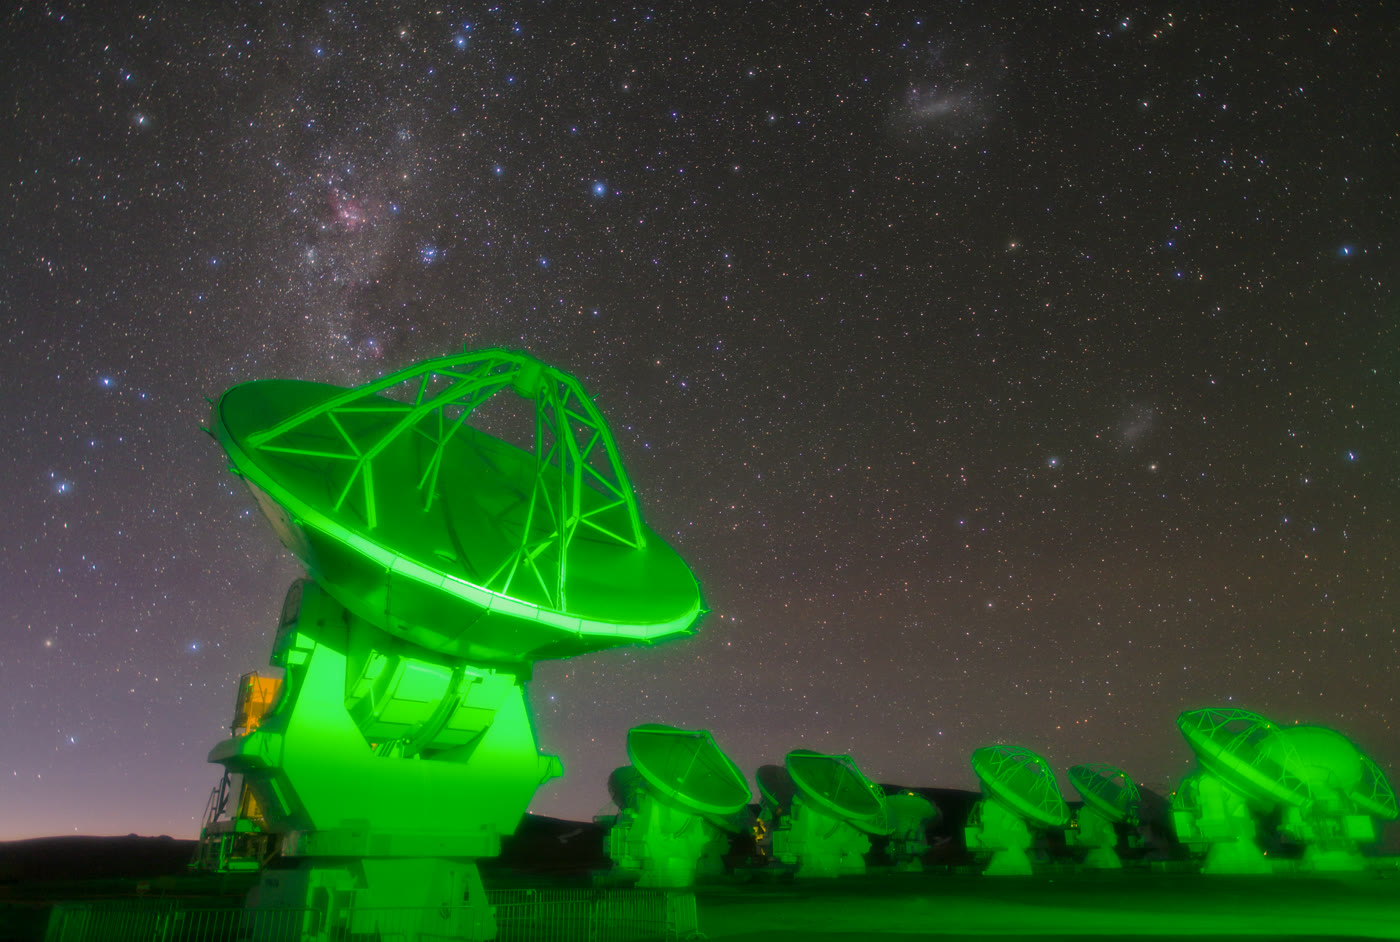
\includegraphics[width=0.7\linewidth]{images/book4/alma-antennas.jpg}

{\small Antenas de um radiointerferômetro em um planalto alto: elas registram,
entre muitas outras, as raias rotacionais do monóxido de carbono das nuvens
interestelares. Fotografia ESO/B.~Tafreshi (twanight.org), CC BY 4.0.}
\end{omfigure}

\section{Espectros rotacionais}

\begin{definition}[Constante rotacional, isotopólogo]\label{def:b3:rovibrational-spectroscopy:rotational-constant}
A \emph{constante rotacional}\index{constante rotacional} de uma molécula linear
é $B = h/(8\pi^2cI)$, em \unit{cm^{-1}} (ou $B = h/8\pi^2I$ em hertz), de modo que
seus níveis rotacionais são $F(J) = BJ(J+1)$ em números de onda. Moléculas que
diferem apenas nos isótopos de seus átomos são \emph{isotopólogos}\index{isotopologo@isotopólogo}
(\ce{^{12}C^{16}O}, \ce{^{13}C^{16}O}); na \omterm{def:b3:computational-chemistry:born-oppenheimer}{aproximação de Born--Oppenheimer},
elas compartilham os mesmos comprimentos de ligação e as mesmas \omterm{def:b3:quantum-model-systems:oscillator}{constantes de força}.
\end{definition}

\begin{definition}[Regras de seleção geral e específica]\label{def:b3:rovibrational-spectroscopy:selection}
Uma \emph{regra de seleção geral}\index{regra de selecao geral@regra de seleção geral} diz que
propriedade uma molécula precisa ter para apresentar um tipo de espectro; uma
\emph{regra de seleção específica}\index{regra de selecao especifica@regra de seleção específica} diz quais
variações de número quântico são permitidas.
\end{definition}

\begin{proposition}[Espectros de rotação pura]\label{prop:b3:rovibrational-spectroscopy:rotational-lines}
Uma molécula só tem espectro de rotação pura (de micro-ondas) se tiver um
momento dipolar permanente; para uma molécula linear, a regra específica é $\Delta J
= \pm1$. As raias de absorção ficam em
\[
\tilde\nu = F(J+1) - F(J) = 2B(J + 1), \qquad J = 0, 1, 2, \dots,
\]
igualmente espaçadas de $2B$.
\end{proposition}

\begin{proof}
A interação com a luz se dá pelo momento dipolar: uma molécula sem dipolo
permanente não tem dipolo oscilante quando gira. A regra $\Delta J
= \pm1$ vem do anulamento de $\int Y_{J'M'}^*\cos\theta\,Y_{JM}$, a menos que $J' = J
\pm 1$ (a componente do dipolo ao longo de $z$ se transforma como $Y_{1,0}$), admitido.
Então $B(J+1)(J+2) - BJ(J+1) = 2B(J+1)$.
\end{proof}

\begin{method}[Comprimento de ligação a partir de uma raia rotacional]\label{met:b3:rovibrational-spectroscopy:bond-length}
\begin{enumerate}
  \item Da raia $J + 1 \leftarrow J$ de frequência $\nu$, deduza $B =
        \nu/2(J+1)$ (em hertz).
  \item Calcule o momento de inércia $I = h/8\pi^2B$.
  \item Com a \omterm{def:b3:quantum-model-systems:oscillator}{massa reduzida} obtida das massas isotópicas, $r = \sqrt{I/\mu}$.
\end{enumerate}
\end{method}

\begin{example}[O monóxido de carbono]\label{ex:b3:rovibrational-spectroscopy:co}
% ledger: rotl:CO.1-0, imass:O16
A raia $J = 1 \leftarrow 0$ de \ce{^{12}C^{16}O} está em \qty{115271.20}{MHz}:
$B = \qty{57635.6}{MHz} = \qty{1.92252}{cm^{-1}}$, $I = \qty{1.4560e-46}{kg.m^2}$.
Com $\mu = 12 \times 15.99491/27.99491 = \qty{6.85621}{u}$, $r_0 = \qty{113.09}{pm}$.
Esse $r_0$ faz a média da ligação sobre sua vibração de ponto zero e é um pouco
mais longo que o comprimento de equilíbrio $r_e$ (\cref{sec:b3:rovibrational-spectroscopy:real-bonds}).
\end{example}

\begin{definition}[Constante de distorção centrífuga]\label{def:b3:rovibrational-spectroscopy:centrifugal}
Uma ligação em rotação se estica; os níveis tornam-se $F(J) = BJ(J+1) - DJ^2(J+1)^2$,
onde $D$ é a \emph{constante de distorção centrífuga}\index{constante de distorcao centrifuga@constante de distorção centrífuga},
e as raias $2B(J+1) - 4D(J+1)^3$ se aproximam lentamente para $J$
alto.
\end{definition}

\begin{proposition}[A raia mais intensa]\label{prop:b3:rovibrational-spectroscopy:jmax}
Se as intensidades das raias seguem a população do nível inferior, $(2J+1)
\eu^{-hcBJ(J+1)/kT}$, o nível mais povoado fica perto de
\[
J_{\max} \approx \sqrt{\frac{kT}{2hcB}} - \frac12.
\]
\end{proposition}

\begin{proof}
Trate $J$ como contínuo e derive: $\frac{\dd}{\dd J}[(2J+1)\eu^{-aJ(J+1)}]
= [2 - a(2J+1)^2]\eu^{-aJ(J+1)}$ com $a = hcB/kT$; a derivada se anula em $(2J + 1)^2 =
2/a$.
\end{proof}

\begin{omfigure}
\begin{tikzpicture}
\begin{axis}[width=0.9\linewidth, height=4.8cm, xmin=0, xmax=70, ymin=0,
  ymax=1.12, ytick=\empty, axis x line=bottom, axis y line=left, ycomb,
  xlabel={número de onda / cm$^{-1}$}, ylabel={intensidade relativa},
  tick label style={font=\small}, label style={font=\small}]
\addplot[omDef, very thick] table[x=nu, y=I] {figdata/out/bachelor-3-rotational-spectrum-co-30.dat};
\addplot[omThm, thick, xshift=1.2pt] table[x=nu, y=I] {figdata/out/bachelor-3-rotational-spectrum-co-300.dat};
\end{axis}
\end{tikzpicture}

{\small O espectro de absorção rotacional do monóxido de carbono, com raias
espaçadas de $2B = \qty{3.845}{cm^{-1}}$ e intensidades tomadas como a população
do nível inferior, a \qty{30}{K} (azul) e a \qty{300}{K} (vermelho, levemente
deslocado para ser visível), cada temperatura normalizada pela sua raia mais
intensa. A \qty{30}{K}, a raia mais intensa é
$J = 3 \leftarrow 2$; a \qty{300}{K}, $J = 8 \leftarrow 7$.}
\end{omfigure}

\section{Vibrações das ligações reais}\label{sec:b3:rovibrational-spectroscopy:real-bonds}

Uma ligação real não obedece à lei de Hooke longe do equilíbrio: ela amolece
quando esticada e se rompe.

\begin{definition}[Potencial de Morse]\label{def:b3:rovibrational-spectroscopy:morse}
O \emph{potencial de Morse}\index{potencial de Morse} é $V(r) = D_e[1 -
\eu^{-\beta(r - r_e)}]^2$: harmônico perto de $r_e$ (\omterm{def:b3:quantum-model-systems:oscillator}{constante de força} $2\beta^2D_e$), e
tendendo ao limite de dissociação $D_e$ para $r$ grande.
\end{definition}

\begin{proposition}[Níveis do oscilador de Morse]\label{prop:b3:rovibrational-spectroscopy:morse-levels}
Em números de onda, os níveis vibracionais de um oscilador de Morse são
\[
G(v) = \tilde\omega_e(v + \tfrac12) - \tilde\omega_ex_e(v + \tfrac12)^2, \qquad
\tilde\omega_ex_e = \frac{\tilde\omega_e^2}{4D_e},
\]
uma escada cujos degraus se aproximam e terminam em $v_{\max} = \lfloor\tilde\omega_e/
2\tilde\omega_ex_e - \frac12\rfloor$.
\end{proposition}
\admitted

A resolução da equação de Morse é tratada em cursos mais avançados; os
níveis são verificados numericamente nos dados das figuras deste capítulo.

\begin{definition}[Constante de anarmonicidade, fundamental, sobretom, banda quente]\label{def:b3:rovibrational-spectroscopy:anharmonic}
$\tilde\omega_ex_e$ é a \emph{constante de anarmonicidade}\index{constante de anarmonicidade}.
A \emph{transição fundamental}\index{transicao fundamental@transição fundamental}
é $v = 1 \leftarrow 0$; um \emph{sobretom}\index{sobretom} é $v = n \leftarrow 0$
com $n \ge 2$, fraco porque a regra geral $\Delta v = \pm1$ do \omterm{def:b3:quantum-model-systems:oscillator}{oscilador
harmônico} é apenas levemente violada; uma \emph{banda quente}\index{banda quente} parte
de um nível excitado, $v = 2 \leftarrow 1$, e cresce com a temperatura.
\end{definition}

\begin{definition}[Energia de dissociação espectroscópica]\label{def:b3:rovibrational-spectroscopy:dissociation}
A \emph{energia de dissociação espectroscópica}\index{energia de dissociacao espectroscopica@energia de dissociação espectroscópica}
de uma molécula é a profundidade de seu potencial, $D_e$, medida a partir do
mínimo, ou $D_0 = D_e - G(0)$, medida a partir do nível mais baixo --- por
molécula, a \qty{0}{K}, ao contrário da entalpia de dissociação de ligação do volume do
2.º ano, uma entalpia molar a \qty{298}{K}.
\end{definition}

\begin{corollary}[$D_e$ e $D_0$ de um oscilador de Morse]\label{cor:b3:rovibrational-spectroscopy:de}
$D_e = \tilde\omega_e^2/4\tilde\omega_ex_e$ e $D_0 = D_e - (\frac12\tilde\omega_e -
\frac14\tilde\omega_ex_e)$.
\end{corollary}

\begin{proof}
A primeira é a relação da proposição; a segunda é $G(0)$.
\end{proof}

\begin{proposition}[Extrapolação de Birge--Sponer]\label{prop:b3:rovibrational-spectroscopy:birge-sponer}
Os intervalos $\Delta G(v + \frac12) = G(v+1) - G(v) = \tilde\omega_e - 2\tilde\omega_ex_e(v +
1)$ diminuem linearmente com $v$; somá-los até que se anulem dá $D_0$, a
área sob o gráfico de $\Delta G$ em função de $v$.
\end{proposition}

\begin{proof}
Subtraia as duas expressões de $G$. $D_0$ é a energia de $v = 0$ até o
limite, a soma de todos os intervalos.
\end{proof}

\begin{example}[O cloreto de hidrogênio]\label{ex:b3:rovibrational-spectroscopy:hcl}
% ledger: diat:HCl.we, diat:HCl.wexe, janaf:H.dfH0, janaf:Cl.dfH0, janaf:HCl.dfH0
Para \ce{H^{35}Cl}, $\tilde\omega_e = \qty{2990.95}{cm^{-1}}$ e $\tilde\omega_ex_e =
\qty{52.82}{cm^{-1}}$: a fundamental está em $\tilde\omega_e - 2\tilde\omega_ex_e =
\qty{2885.3}{cm^{-1}}$ e o primeiro \omterm{def:b3:rovibrational-spectroscopy:anharmonic}{sobretom} em $2\tilde\omega_e - 6\tilde\omega_ex_e =
\qty{5665.0}{cm^{-1}}$, um pouco menos que o dobro da fundamental. O modelo de Morse
prevê $D_e = \qty{42342}{cm^{-1}}$ e $D_0 = \qty{40860}{cm^{-1}}$; o $D_0$ verdadeiro,
obtido das entalpias de formação de H, Cl e HCl a \qty{0}{K}, é
\qty{35760}{cm^{-1}} (\qty{4.43}{eV}). O potencial real se achata mais depressa que uma
curva de Morse ajustada no fundo: as extrapolações de Birge--Sponer a partir dos
níveis mais baixos superestimam as energias de dissociação.
\end{example}

\begin{omfigure}
\begin{tikzpicture}
\begin{axis}[name=morse, width=0.55\linewidth, height=6cm, xmin=0.8, xmax=4.0,
  ymin=0, ymax=48000, axis lines=left, xlabel={$r$ / \AA}, ylabel={$V$ / cm$^{-1}$},
  unbounded coords=jump, scaled y ticks=false, ytick={0,10000,20000,30000,40000},
  tick label style={font=\small}, label style={font=\small}]
\addplot[black, thick] table[x=r, y=V] {figdata/out/bachelor-3-morse-levels.dat};
\addplot[gray, dashed] table[x=r, y=harm] {figdata/out/bachelor-3-morse-levels.dat};
\addplot[omDef] table[x=r, y=E] {figdata/out/bachelor-3-morse-levels-levels.dat};
\draw[<->, omThm] (axis cs:3.7,0) -- (axis cs:3.7,42342) node[pos=0.5, left, font=\small] {$D_e$};
\draw[dashed, omThm] (axis cs:1.2,42342) -- (axis cs:4.0,42342);
\end{axis}
\begin{axis}[at={(morse.east)}, anchor=west, xshift=1.6cm, width=0.4\linewidth,
  height=5cm, xmin=0, xmax=28, ymin=0, ymax=3100, axis lines=left,
  xlabel={$v$}, ylabel={$\Delta G(v + \frac12)$ / cm$^{-1}$},
  tick label style={font=\small}, label style={font=\small}]
\addplot[omDef, only marks, mark size=1.2pt] table[x=v, y=dG] {figdata/out/bachelor-3-morse-levels-bs.dat};
\addplot[omDef!40, fill=omDef!12, draw=none] table[x=v, y=dG] {figdata/out/bachelor-3-morse-levels-bs.dat} \closedcycle;
\end{axis}
\end{tikzpicture}

{\small À esquerda: o \omterm{def:b3:rovibrational-spectroscopy:morse}{potencial de Morse} de \ce{HCl} construído a partir de suas
constantes espectroscópicas (traço contínuo), a parábola harmônica de mesma
curvatura (tracejada) e um a cada três níveis vibracionais, desenhados entre
seus pontos de retorno; os níveis se aproximam de $D_e$. À direita: o gráfico
de Birge--Sponer dos intervalos; a área sombreada é $D_0$.}
\end{omfigure}

\section{Bandas rovibracionais}

Uma transição vibracional de um gás é acompanhada de variações rotacionais, $\Delta
J = \pm1$ para uma diatômica em um estado ${}^1\Sigma$.

\begin{definition}[Ramos P, Q e R, origem da banda]\label{def:b3:rovibrational-spectroscopy:branches}
Em uma banda rovibracional, as raias com $\Delta J = -1$ formam o \emph{ramo
P}\index{ramo P}, as com $\Delta J = +1$ o \emph{ramo R}\index{ramo R},
e as com $\Delta J = 0$, quando permitidas, o \emph{ramo Q}\index{ramo Q}.
A \emph{origem da banda}\index{origem da banda} $\tilde\nu_0$ é a
diferença de energia vibracional sem rotação.
\end{definition}

\begin{theorem}[Diferenças de combinação]\label{thm:b3:rovibrational-spectroscopy:combination-differences}
Com as \omterm{def:b3:rovibrational-spectroscopy:rotational-constant}{constantes rotacionais} $B_0$ e $B_1$ nos níveis vibracionais inferior e
superior, $R(J) = \tilde\nu_0 + B_1(J+1)(J+2) - B_0J(J+1)$ e $P(J) = \tilde\nu_0 +
B_1(J-1)J - B_0J(J+1)$, e
\[
R(J - 1) - P(J + 1) = 4B_0(J + \tfrac12), \qquad R(J) - P(J) = 4B_1(J + \tfrac12).
\]
\end{theorem}

\begin{proof}
As duas primeiras decorrem de $E = G(v) + B_vJ(J+1)$ para os dois níveis. $R(J - 1)$ e
$P(J + 1)$ terminam no mesmo nível superior $J$, partindo dos níveis inferiores $J - 1$ e $J + 1$:
sua diferença é $B_0[(J+1)(J+2) - (J-1)J] = B_0(4J + 2)$. Do mesmo modo, $R(J)$ e
$P(J)$ partem do mesmo nível inferior e terminam em $J + 1$ e $J - 1$.
\end{proof}

\begin{method}[Analisar uma banda rovibracional]\label{met:b3:rovibrational-spectroscopy:combination}
\begin{enumerate}
  \item Localize a lacuna: para uma diatômica ${}^1\Sigma$ não há \omterm{def:b3:rovibrational-spectroscopy:branches}{ramo Q}, e
        $\tilde\nu_0$ fica na lacuna, entre $R(0)$ e $P(1)$.
  \item Numere as raias a partir da lacuna, para fora: $R(0), R(1), \dots$ e $P(1),
        P(2), \dots$.
  \item Use as diferenças de combinação para obter $B_0$ e $B_1$
        separadamente, e depois $\alpha_e = B_0 - B_1$ e $B_e = B_0 + \frac12\alpha_e$.
\end{enumerate}
\end{method}

\begin{omfigure}
\begin{tikzpicture}
\begin{axis}[width=0.92\linewidth, height=5cm, xmin=2650, xmax=3080, ymin=0,
  ymax=1.15, ytick=\empty, axis x line=bottom, axis y line=left,
  xlabel={número de onda / cm$^{-1}$}, ylabel={absorbância (relativa)},
  tick label style={font=\small}, label style={font=\small}]
\addplot[omDef, thin] table[x=nu, y=A] {figdata/out/bachelor-3-rovib-band.dat};
\node[font=\small] at (axis cs:2780,1.06) {ramo P};
\node[font=\small] at (axis cs:2985,1.06) {ramo R};
\draw[->, gray] (axis cs:2885.3,0.45) -- (axis cs:2885.3,0.05);
\node[font=\small, gray, anchor=south] at (axis cs:2885.3,0.45) {$\tilde\nu_0$};
\end{axis}
\end{tikzpicture}

{\small A banda fundamental de \ce{HCl} gasoso a \qty{300}{K}, calculada a partir
de suas constantes espectroscópicas: \omterm{def:b3:rovibrational-spectroscopy:branches}{ramos P} e R de cada lado da lacuna na
\omterm{def:b3:rovibrational-spectroscopy:branches}{origem da banda}. Cada raia é um dubleto, \ce{H^{35}Cl} e o mais fraco, um pouco
mais baixo, \ce{H^{37}Cl} (abundâncias naturais de 76\,\% e 24\,\%). As raias R se
aproximam e as raias P se afastam, porque $B_1 < B_0$.}
\end{omfigure}

\begin{example}[As constantes de \ce{HCl} a partir de sua banda]\label{ex:b3:rovibrational-spectroscopy:analysis}
% ledger: diat:HCl.Be, diat:HCl.ae
Com $R(0) = \qty{2905.58}{cm^{-1}}$ e $P(2) = \qty{2842.94}{cm^{-1}}$, encontra-se
$6B_0 = \qty{62.64}{cm^{-1}}$, logo $B_0 = \qty{10.440}{cm^{-1}}$. Com $R(1) = 2925.23$ e $P(1) =
\qty{2864.43}{cm^{-1}}$, $B_1 = \qty{10.133}{cm^{-1}}$. Logo $\alpha_e = \qty{0.307}{cm^{-1}}$
e $B_e = \qty{10.593}{cm^{-1}}$, os valores a partir dos quais a banda foi construída:
o método os recupera exatamente.
\end{example}

\section{Espectroscopia Raman}

\begin{definition}[Espalhamento Raman e Rayleigh]\label{def:b3:rovibrational-spectroscopy:raman}
Quando luz de frequência $\nu_0$ atravessa uma amostra, a maior parte da luz
espalhada conserva a frequência $\nu_0$: é o \emph{espalhamento Rayleigh}\index{espalhamento Rayleigh}.
Uma pequena fração é deslocada pelas frequências rotacionais ou vibracionais
das moléculas: é o \emph{espalhamento Raman}\index{espalhamento Raman}.
As raias de frequência mais baixa são as \emph{raias Stokes}\index{raia Stokes} (a
molécula ganhou energia), as de frequência mais alta, as \emph{raias
anti-Stokes}\index{raia anti-Stokes} (ela perdeu energia).
\end{definition}

\begin{proposition}[Origem clássica do efeito Raman]\label{prop:b3:rovibrational-spectroscopy:raman-classical}
Se a polarizabilidade de uma molécula que vibra em $\nu_{\mathrm{vib}}$ varia
como $\alpha = \alpha_0 + \alpha_1\cos(2\pi\nu_{\mathrm{vib}}t)$, o dipolo induzido por um
campo $E_0\cos(2\pi\nu_0t)$ oscila em $\nu_0$ e em $\nu_0 \pm \nu_{\mathrm{vib}}$.
Uma vibração só é \omterm{def:b3:group-theory-applied:activity}{ativa no Raman} se alterar a polarizabilidade.
\end{proposition}

\begin{proof}
$\mu = \alpha E = \alpha_0E_0\cos(2\pi\nu_0t) + \frac12\alpha_1E_0[\cos2\pi(\nu_0 +
\nu_{\mathrm{vib}})t + \cos2\pi(\nu_0 - \nu_{\mathrm{vib}})t]$, por $\cos a\cos b =
\frac12[\cos(a+b) + \cos(a-b)]$. Cada dipolo oscilante irradia em sua própria
frequência; sem $\alpha_1$, só resta o termo Rayleigh.
\end{proof}

\begin{proposition}[Raias Raman rotacionais]\label{prop:b3:rovibrational-spectroscopy:rotational-raman}
Uma molécula linear com polarizabilidade anisotrópica apresenta raias Raman
rotacionais com $\Delta J = \pm2$, deslocadas em relação à raia excitadora de
\[
|\Delta\tilde\nu| = F(J+2) - F(J) = 4B(J + \tfrac32) = 6B, 10B, 14B, \dots
\]
--- a primeira raia em $6B$, depois um espaçamento de $4B$.
\end{proposition}

\begin{proof}
O elipsoide de polarizabilidade de uma molécula linear em rotação volta à
mesma orientação duas vezes por volta, logo modula o espalhamento com o dobro
da frequência de rotação: $\Delta J = \pm2$ (a regra quântica, admitida). Então
$B(J+2)(J+3) - BJ(J+1) = B(4J + 6)$.
\end{proof}

\begin{example}[O nitrogênio visto pelo Raman]\label{ex:b3:rovibrational-spectroscopy:n2}
% ledger: diat:N2.Be, diat:N2.ae
\ce{N2} não tem dipolo nem espectro de infravermelho ou de micro-ondas, mas sua
polarizabilidade é anisotrópica: suas raias Raman rotacionais começam a $6B_0 =
\qty{11.94}{cm^{-1}}$ da raia excitadora e são espaçadas de \qty{7.96}{cm^{-1}}. Suas
intensidades alternam na razão 2:1 entre $J$ par e ímpar: os dois núcleos \ce{^{14}N} são
idênticos, e a estatística de spin nuclear (\cref{ch:b3:statistical-thermo-applied})
dá aos níveis de $J$ par o dobro do peso dos ímpares.
\end{example}

\begin{omfigure}
\begin{tikzpicture}
\begin{axis}[name=r, width=0.55\linewidth, height=4.6cm, xmin=-110, xmax=110,
  ymin=0, ymax=1.1, ytick=\empty, axis x line=bottom, axis y line=left, ycomb,
  xlabel={deslocamento Raman / cm$^{-1}$}, tick label style={font=\small}, label style={font=\small},
  title={\small \ce{N2}, Raman rotacional, \qty{300}{K}}]
\addplot[omDef, thick] table[x=shift, y=I] {figdata/out/bachelor-3-rotational-spectrum-n2-raman.dat};
\draw[gray, thick] (axis cs:0,0) -- (axis cs:0,1.05);
\end{axis}
\begin{scope}[xshift=0.6\linewidth, font=\small]
  \draw[omstate] (0,0) -- (2.4,0) node[right] {$v = 0$};
  \draw[omstate] (0,1.0) -- (2.4,1.0) node[right] {$v = 1$};
  \draw[omvib, densely dashed] (0,3.2) -- (2.4,3.2) node[right] {virtual};
  \draw[omabs] (0.3,0) -- (0.3,3.18);
  \draw[omfluo] (0.5,3.18) -- (0.5,0.02);
  \node[font=\scriptsize, omThm, anchor=east] at (0.22,1.6) {Rayleigh};
  \draw[omabs] (1.3,0) -- (1.3,3.18);
  \draw[omphos] (1.5,3.18) -- (1.5,1.02) node[pos=0.4, right, font=\scriptsize] {Stokes};
\end{scope}
\end{tikzpicture}

{\small À esquerda: o espectro Raman rotacional do nitrogênio calculado a
\qty{300}{K}: \omterm{def:b3:rovibrational-spectroscopy:raman}{raias Stokes} nos deslocamentos positivos (à direita), \omterm{def:b3:rovibrational-spectroscopy:raman}{raias anti-Stokes}
nos deslocamentos negativos (à esquerda, um pouco mais fracas), com a alternância
2:1 das intensidades; a linha cinza em zero marca a raia Rayleigh, muito mais
intensa. À direita: esquema de energia do \omterm{def:b3:rovibrational-spectroscopy:raman}{espalhamento Rayleigh} e Stokes através
de um nível virtual (que não é um estado real da molécula).}
\end{omfigure}

\section{Moléculas poliatômicas}

\begin{definition}[Tipos de rotores]\label{def:b3:rovibrational-spectroscopy:rotor-types}
Uma molécula com três momentos principais de inércia iguais é um
\emph{pião esférico}\index{piao esferico@pião esférico} (\ce{CH4}, \ce{SF6}); com dois iguais, um
\emph{pião simétrico}\index{piao simetrico@pião simétrico} (\ce{NH3}, \ce{CHCl3}, \ce{C6H6});
com os três diferentes, um \emph{pião assimétrico}\index{piao assimetrico@pião assimétrico}
(\ce{H2O}, a maioria das moléculas); as moléculas lineares têm um momento nulo.
\end{definition}

Um \omterm{def:b3:rovibrational-spectroscopy:rotor-types}{pião esférico} não tem dipolo nem espectro rotacional; um \omterm{def:b3:rovibrational-spectroscopy:rotor-types}{pião simétrico} tem
os níveis $BJ(J+1) + (A - B)K^2$, onde $K$ conta o momento angular em torno de seu eixo,
e raias que ainda caem em $2B(J+1)$, pois $\Delta K = 0$; um \omterm{def:b3:rovibrational-spectroscopy:rotor-types}{pião assimétrico}
tem um espectro irregular, ajustado por computador. As vibrações das moléculas
poliatômicas são seus \omterm{def:b3:group-theory-applied:normal-mode}{modos normais}, rotulados e selecionados pelo
\cref{ch:b3:group-theory-applied}: o espectro de infravermelho mostra os modos
que se transformam como $x$, $y$, $z$, cada um com sua própria estrutura rotacional.

\begin{inthelab}[Uma célula de gás em um espectrômetro de infravermelho]
\ce{HCl} gasoso é admitido em uma célula de \qty{10}{cm} com janelas transparentes
no infravermelho, dentro de um espectrômetro de transformada de Fourier. Com
resolução de \qty{1}{cm^{-1}}, os \omterm{def:b3:rovibrational-spectroscopy:branches}{ramos P} e R aparecem como raias simples; com
\qty{0.25}{cm^{-1}}, cada uma se desdobra em seu dubleto \ce{H^{35}Cl}/\ce{H^{37}Cl},
separado por \qty{2}{cm^{-1}}. O cloreto de hidrogênio é tóxico e corrosivo: a
célula é carregada em uma linha de vácuo, dentro da capela.
\end{inthelab}

\begin{safety}{\ghs[0.8cm]{GHS04}\ghs[0.8cm]{GHS05}\ghs[0.8cm]{GHS06}}
Cloreto de hidrogênio gasoso: gás sob pressão, corrosivo para a pele, os olhos e
as vias respiratórias, tóxico por inalação. Manipulado apenas em aparelhagem
fechada ou na capela.
\end{safety}

\begin{history}[Raman, 1928]
Em 1928, C. V. Raman e K. S. Krishnan observaram, na luz solar filtrada por um
filtro violeta e espalhada por líquidos, uma luz fraca de outra cor, que um
filtro verde cruzado conseguia isolar. Raman recebeu o Prêmio Nobel de Física
de 1930; as fontes laser transformaram seu efeito em uma técnica analítica de
rotina cinquenta anos depois.
\end{history}

\section{Exercícios}

\begin{exercise}[$\star$]\label{exo:b3:rovibrational-spectroscopy:1}
% ledger: imass:O16
A partir de $B_0 = \qty{1.9225}{cm^{-1}}$ para \ce{^{12}C^{16}O}, calcule o momento de
inércia e o comprimento de ligação $r_0$.
\end{exercise}

\begin{exercise}[$\star$]\label{exo:b3:rovibrational-spectroscopy:2}
% ledger: diat:HCl.Be, diat:HCl.ae
Com $B_0 = \qty{10.440}{cm^{-1}}$, dê as posições das quatro primeiras raias do
espectro rotacional de \ce{H^{35}Cl} e o $J$ da raia mais intensa a
\qty{300}{K}.
\end{exercise}

\begin{exercise}[$\star$]\label{exo:b3:rovibrational-spectroscopy:3}
Quais entre \ce{H2}, \ce{HCl}, \ce{N2}, \ce{CO2}, \ce{CH4}, \ce{SF6} e \ce{H2O} apresentam um
espectro de absorção de rotação pura? Um espectro Raman rotacional?
\end{exercise}

\begin{exercise}[$\star$]\label{exo:b3:rovibrational-spectroscopy:4}
% ledger: diat:HCl.we, diat:HCl.wexe
Que fração das moléculas de \ce{HCl} está em $v = 1$ a 300 e a \qty{1000}{K}
(fundamental em \qty{2885.3}{cm^{-1}})? Quando a \omterm{def:b3:rovibrational-spectroscopy:anharmonic}{banda quente} se torna visível?
\end{exercise}

\begin{exercise}[$\star\star$]\label{exo:b3:rovibrational-spectroscopy:5}
A fundamental e o primeiro \omterm{def:b3:rovibrational-spectroscopy:anharmonic}{sobretom} de \ce{H^{35}Cl} ficam em 2885.3 e
\qty{5665.0}{cm^{-1}}. Deduza $\tilde\omega_e$ e $\tilde\omega_ex_e$.
\end{exercise}

\begin{exercise}[$\star\star$]\label{exo:b3:rovibrational-spectroscopy:6}
Com as constantes do exercício anterior, calcule $D_e$ e $D_0$ do modelo de
Morse e compare com o valor verdadeiro $D_0 = \qty{35760}{cm^{-1}}$. Converta os dois
valores de $D_0$ em \unit{kJ/mol}.
\end{exercise}

\begin{exercise}[$\star\star$]\label{exo:b3:rovibrational-spectroscopy:7}
Quatro raias da fundamental de \ce{H^{35}Cl} são $R(0) = 2905.58$, $R(1) = 2925.23$,
$P(1) = 2864.43$ e $P(2) = \qty{2842.94}{cm^{-1}}$. Encontre $B_0$, $B_1$, $\alpha_e$ e
a \omterm{def:b3:rovibrational-spectroscopy:branches}{origem da banda}.
\end{exercise}

\begin{exercise}[$\star\star$]\label{exo:b3:rovibrational-spectroscopy:8}
% ledger: imass:H1, imass:H2, imass:Cl35
Preveja $B_0$ e a \omterm{def:b3:rovibrational-spectroscopy:branches}{origem da banda} de \ce{D^{35}Cl} a partir dos de \ce{H^{35}Cl}, usando
as \omterm{def:b3:quantum-model-systems:oscillator}{massas reduzidas} ($\tilde\omega_e \propto \mu^{-1/2}$, $\tilde\omega_ex_e \propto
\mu^{-1}$, $B \propto \mu^{-1}$).
\end{exercise}

\begin{exercise}[$\star\star$]\label{exo:b3:rovibrational-spectroscopy:9}
% ledger: diat:N2.Be, diat:N2.ae
Para \ce{N2}, $B_0 = \qty{1.9896}{cm^{-1}}$. Dê os deslocamentos das três primeiras
raias Raman rotacionais Stokes e explique a alternância de suas
intensidades.
\end{exercise}

\begin{exercise}[$\star\star\star$]\label{exo:b3:rovibrational-spectroscopy:10}
% ledger: rotl:CO.1-0, rotl:CO.2-1, rotl:CO.3-2
As três primeiras raias rotacionais de \ce{^{12}C^{16}O} estão em 115271.2018,
230538.0000 e \qty{345795.9899}{MHz}. Mostre que um \omterm{def:b3:quantum-model-systems:rotor}{rotor rígido} não as ajusta e
determine $B$ e a \omterm{def:b3:rovibrational-spectroscopy:centrifugal}{constante de distorção centrífuga} $D$.
\end{exercise}

\begin{exercise}[$\star\star\star$]\label{exo:b3:rovibrational-spectroscopy:11}
Mostre que a soma de Birge--Sponer dos intervalos $\Delta G(v + \frac12)$ de um
oscilador de Morse, de $v = 0$ até o último nível ligado, é próxima de $D_e - G(0)$, e
avalie a soma para \ce{HCl}.
\end{exercise}

\begin{exercise}[$\star\star\star$]\label{exo:b3:rovibrational-spectroscopy:12}
O núcleo \ce{^{16}O} tem spin nulo, de modo que os níveis de \ce{^{16}O^{12}C^{16}O}
com $J$ ímpar não existem. Qual é o espaçamento de suas raias Raman rotacionais, e o
deslocamento da primeira, em função de $B$? Por que \ce{CO2} não tem espectro de
micro-ondas?
\end{exercise}

\section{Problema: Escutando uma nuvem fria}

\begin{problem}[{Problema de fim de semana --- o comprimento da ligação do monóxido de
carbono a partir de sua primeira raia rotacional, a temperatura de uma nuvem
interestelar, o isotopólogo de carbono 13 e a banda de infravermelho}]
\label{pb:b3:rovibrational-spectroscopy:1}
% ledger: rotl:CO.1-0, rotl:CO.2-1, rotl:13CO.1-0, imass:O16, imass:C13, iso:C13, diat:CO.we, diat:CO.wexe, re:CO
Dados: raias de \ce{^{12}C^{16}O} $J = 1 \leftarrow 0$ em \qty{115.2712}{GHz} e $2
\leftarrow 1$ em \qty{230.5380}{GHz}; raia $1 \leftarrow 0$ de \ce{^{13}C^{16}O} em
\qty{110.2014}{GHz}; massas \ce{^{12}C} 12 (exatamente), \ce{^{13}C} 13.00335,
\ce{^{16}O} \qty{15.99491}{u}; abundância natural de \ce{^{13}C} 1.1\,\%; para \ce{^{12}C^{16}O},
$\tilde\omega_e = \qty{2169.81}{cm^{-1}}$, $\tilde\omega_ex_e = \qty{13.288}{cm^{-1}}$, e o
comprimento de equilíbrio $r_e = \qty{112.83}{pm}$. $h = \qty{6.62607e-34}{J.s}$, $u =
\qty{1.66054e-27}{kg}$, $c = \qty{2.99792e10}{cm/s}$, $hc/k = \qty{1.43878}{cm.K}$.

\medskip\noindent\textbf{Parte I --- A ligação.}
\begin{enumerate}
  \item Calcule $B_0$ em hertz e em \unit{cm^{-1}}.
  \item Calcule a \omterm{def:b3:quantum-model-systems:oscillator}{massa reduzida} de \ce{^{12}C^{16}O} em quilogramas.
  \item Calcule o momento de inércia.
  \item Deduza $r_0$.
  \item Compare com $r_e$. Por que $r_0$ é mais longo?
  \item Preveja a raia $2 \leftarrow 1$ para um \omterm{def:b3:quantum-model-systems:rotor}{rotor rígido}. Comente o
        valor medido.
\end{enumerate}

\medskip\noindent\textbf{Parte II --- A temperatura da nuvem.}
\begin{enumerate}[resume]
  \item Dê as energias, em \unit{cm^{-1}} e em kelvins ($E/k$), dos níveis $J =
        0$, 1, 2.
  \item Escreva a razão das populações $N_2/N_1$ à temperatura $T$.
  \item As observações dão $N_2/N_1 = 0.85$ (dados do problema). Encontre $T$.
  \item Que nível é o mais povoado a essa temperatura?
  \item Por que uma nuvem assim não pode ser vista na banda vibracional de infravermelho?
  \item Por que a raia $1 \leftarrow 0$ é o traçador de gás frio mais usado?
\end{enumerate}

\medskip\noindent\textbf{Parte III --- O \omterm{def:b3:rovibrational-spectroscopy:rotational-constant}{isotopólogo}.}
\begin{enumerate}[resume]
  \item Calcule a \omterm{def:b3:quantum-model-systems:oscillator}{massa reduzida} de \ce{^{13}C^{16}O}.
  \item Preveja sua raia $1 \leftarrow 0$ a partir da de \ce{^{12}C^{16}O}.
  \item Compare com os \qty{110.2014}{GHz} medidos. O que foi desprezado?
  \item Se as duas raias fossem fracas e não saturadas, que razão de suas
        intensidades as abundâncias naturais dariam?
  \item A razão observada é muito menor. O que isso diz sobre a raia de
        \ce{^{12}C^{16}O}?
  \item Por que os dois \omterm{def:b3:rovibrational-spectroscopy:rotational-constant}{isotopólogos} são observados juntos na prática?
\end{enumerate}

\medskip\noindent\textbf{Parte IV --- A banda vibracional.}
\begin{enumerate}[resume]
  \item Calcule a \omterm{def:b3:rovibrational-spectroscopy:branches}{origem da banda} fundamental, em \unit{cm^{-1}} e em
        micrômetros.
  \item Calcule o primeiro \omterm{def:b3:rovibrational-spectroscopy:anharmonic}{sobretom}.
  \item Calcule a \omterm{def:b3:quantum-model-systems:oscillator}{energia do ponto zero}.
  \item O que separa as primeiras raias R e P?
  \item Que molécula, \ce{^{12}C^{16}O} ou \ce{^{13}C^{16}O}, tem a origem de banda mais baixa?
  \item Enuncie o resultado: o comprimento de ligação $r_0$ do monóxido de carbono
        obtido a partir de uma única raia de rádio.
\end{enumerate}
\end{problem}
